\chapter{Landasan Perancangan dan Pengembangan Kurikulum}

\reviewfrompdf{Uraian Landasan Filosofis, Sosiologis, Psikologis, dan Yuridis pada bab ini diperkaya berdasarkan Dokumen Kurikulum D4 Teknik Informatika 2020. Redaksi dan referensi hukum perlu ditinjau ulang oleh tim kurikulum sebelum dokumen dinyatakan final.}

\section{Landasan Filosofis}

Pembelajaran adalah inti dari kurikulum sedangkan kurikulum adalah inti dari pendidikan. Operasionalisasi pendidikan dan kurikulum terletak pada kegiatan pembelajaran yang memosisikan dosen sebagai fasilitator proses belajar mahasiswa.

\begin{figure}[H]
\centering
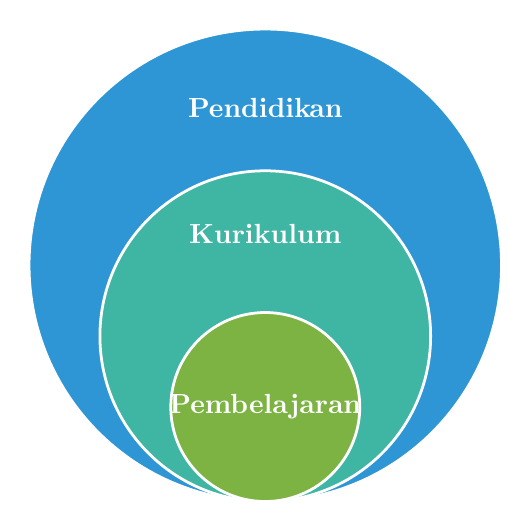
\begin{tikzpicture}
\definecolor{lingkpendidikan}{HTML}{2E96D5}
\definecolor{lingkkurikulum}{HTML}{3FB5A3}
\definecolor{lingkpembelajaran}{HTML}{7CB342}
\filldraw[lingkpendidikan, draw=white, line width=1pt] (0,3) circle (3cm);
\filldraw[lingkkurikulum, draw=white, line width=1pt] (0,2.1) circle (2.1cm);
\filldraw[lingkpembelajaran, draw=white, line width=1pt] (0,1.2) circle (1.2cm);
\node[text=white, font=\bfseries] at (0,5) {Pendidikan};
\node[text=white, font=\bfseries] at (0,3.4) {Kurikulum};
\node[text=white, font=\bfseries] at (0,1.2) {Pembelajaran};
\end{tikzpicture}
\caption{Posisi Pembelajaran dalam Konteks Pendidikan}
\end{figure}

\paragraph{Posisi Pembelajaran dalam Pendidikan} Implementasi Merdeka Belajar sejalan dengan filosofi demokrasi pendidikan, di mana mahasiswa diberi ruang untuk menentukan pilihan sumber belajar, cara belajar, dan konteks pengembangan dirinya.

\paragraph{Pandangan Paulo Freire} Paulo Freire, tokoh demokrasi pendidikan, memandang bahwa manusia itu berproses dan belum selesai (belum utuh). Pendidikan diarahkan untuk membentuk manusia yang otonom terhadap dirinya, terbebas dari tekanan, dan memiliki dasar hidup yang jelas dan realistis. Keutuhan tersebut dicapai melalui kesadaran diri yang diperoleh dari kebebasan. Dalam proses pembelajaran, dosen dan mahasiswa secara hakiki tidak berbeda: keduanya berada dalam proses dinamis \emph{on becoming} (untuk menjadi). Dosen sebagai pendidik sekaligus salah satu sumber belajar, sehingga masih banyak sumber belajar lain yang dapat dipilih mahasiswa; konsekuensinya, dosen berkewajiban memberi keleluasaan kepada mahasiswa dalam menentukan pilihan sumber, cara, dan tempat belajar yang sesuai dengan minatnya.

\paragraph{Asumsi Filosofis Pembelajaran} Terdapat tiga asumsi filosofis yang dikembangkan dalam pembelajaran:
\begin{enumerate}
\item Pembelajaran adalah proses berpikir untuk mencari dan menemukan, bukan sekadar diajari. Implementasinya diarahkan pada pembentukan keterampilan mental tertentu seperti keterampilan berpikir kritis dan berpikir kreatif (\emph{teaching of thinking}).
\item Usaha menciptakan lingkungan belajar yang mendorong pengembangan kognitif, seperti menciptakan suasana keterbukaan yang demokratis dan iklim belajar yang menyenangkan (\emph{teaching for thinking}).
\item Upaya membantu peserta didik agar lebih sadar terhadap proses berpikirnya sendiri (\emph{teaching about thinking}).
\end{enumerate}

\paragraph{Pendidikan sebagai Transfer Nilai} Perguruan tinggi tidak hanya berfungsi memindahkan pengetahuan (\emph{transfer of knowledge}), tetapi juga memindahkan nilai (\emph{transfer of value}), sehingga lulusan menjadi terampil, berintelektual baik, dan memiliki internalisasi nilai dalam wujud karakter.

\section{Landasan Sosiologis}

Kurikulum dikembangkan berdasarkan budaya bangsa Indonesia yang beragam, diarahkan untuk membangun kehidupan masa kini, dan menjadi dasar bagi kehidupan bangsa yang lebih baik di masa depan.

Kurikulum perlu merespons perubahan sosial, perkembangan IPTEK, kebutuhan masyarakat, dan keterampilan abad 21, serta memberi kebebasan bagi peserta didik untuk memperkaya kompetensi melalui pengalaman belajar yang relevan. Secara lebih rinci, landasan sosiologis pengembangan kurikulum Program Studi D4 Teknik Informatika mencakup:
\begin{enumerate}
\item Kurikulum mampu merespons perubahan sosial dari perkembangan masyarakat yang dipengaruhi oleh falsafah hidup, nilai-nilai, IPTEK, dan kebutuhan yang ada dalam masyarakat, sehingga menuntut tersedianya proses pendidikan yang relevan.
\item Kurikulum tersusun atas sistem yang progresif, mencakup mutu pendidikan dalam konteks \emph{input}, \emph{process}, \emph{output}, dan \emph{outcome}, agar tercipta lulusan yang terampil, produktif, loyal, dan adaptif.
\item Keterampilan abad 21 menjadi tuntutan lingkungan internasional untuk meningkatkan \emph{literacy}, \emph{numeracy}, \emph{scientific literacy}, \emph{ICT literacy}, \emph{financial literacy}, serta \emph{cultural and civic literacy}.
\item Peserta didik memiliki kebebasan untuk mengembangkan diri dengan memperkaya kompetensi melalui pengalaman pembelajaran baru pada lingkungan praktis yang beragam secara terstruktur dan sistematis, yang diwujudkan melalui program Merdeka Belajar Kampus Merdeka (MBKM).
\end{enumerate}

\section{Landasan Psikologis}

Kebijakan Merdeka Belajar bertujuan mewujudkan proses pembelajaran yang otonom dan fleksibel sehingga tercipta kultur belajar yang inovatif, tidak mengekang, dan sesuai dengan kebutuhan mahasiswa.

Kebijakan ini juga bertujuan meningkatkan \emph{link and match} dengan dunia usaha dan dunia industri, serta mempersiapkan mahasiswa memasuki dunia kerja sejak awal. Melalui program MBKM, mahasiswa diberikan kebebasan mengambil satuan kredit semester (sks) pembelajaran di luar program studi selama tiga semester, baik di dalam maupun di luar perguruan tinggi, dengan orientasi capaian pembelajaran secara utuh.

Penguatan pendidikan karakter perlu menyertai pembelajaran melalui pengembangan \emph{computational thinking}, \emph{creativity}, \emph{critical thinking}, \emph{collaboration}, \emph{communication}, dan \emph{compassion}. Penguatan Pendidikan Karakter (PPK) menjadi kebijakan yang wajib menyertai Merdeka Belajar, dengan payung hukum Peraturan Menteri Pendidikan dan Kebudayaan Nomor 20 Tahun 2018 tentang Penguatan Pendidikan Karakter pada Satuan Pendidikan Formal.

PPK dilakukan dengan berbasis pada kearifan lokal sebagai strategi revitalisasi nilai-nilai Pancasila untuk menguatkan karakter dan jati diri bangsa, dengan didasari oleh:
\begin{enumerate}
\item Integrasi kearifan lokal budaya yang bersumber dari \emph{core value} hormat, rukun, dan tolong-menolong sebagai strategi revitalisasi nilai-nilai Pancasila dan nilai karakter.
\item Persiapan peserta didik sebagai warga negara yang cerdas dan baik, melalui pembelajaran sambil berbuat, belajar memecahkan masalah sosial, belajar melalui pelibatan sosial, serta belajar melalui pembiasaan dan interaksi sosial-kultural.
\item Implementasi model pembelajaran yang dikembangkan dengan pendekatan \emph{Problem Based Learning}, \emph{Project Based Learning}, dan klarifikasi nilai.
\end{enumerate}

\section{Landasan Yuridis}

Merdeka Belajar menjadi salah satu upaya strategis pemerintah dalam bidang pendidikan, yang diperkuat oleh sejumlah peraturan sebagai landasan hukum penyusunan kurikulum:

\begin{enumerate}
\item Undang-Undang Dasar Negara Republik Indonesia Tahun 1945 Bab XIII Pasal 31 ayat (1): setiap warga negara berhak mendapat pendidikan.
\item Peraturan Presiden Nomor 8 Tahun 2012 tentang Kerangka Kualifikasi Nasional Indonesia (KKNI).
\item Undang-Undang Nomor 12 Tahun 2012 tentang Pendidikan Tinggi:
  \begin{enumerate}
  \item Sistem pendidikan nasional yang meningkatkan keimanan, ketakwaan kepada Tuhan Yang Maha Esa, dan akhlak mulia dalam rangka mencerdaskan kehidupan bangsa serta memajukan ilmu pengetahuan dan teknologi dengan menjunjung tinggi nilai-nilai agama dan persatuan bangsa.
  \item Pendidikan tinggi sebagai bagian dari sistem pendidikan nasional memiliki peran strategis dalam mencerdaskan kehidupan bangsa dan memajukan ilmu pengetahuan dan teknologi dengan memperhatikan dan menerapkan nilai humaniora.
  \item Pendidikan tinggi yang mampu mengembangkan ilmu pengetahuan dan teknologi serta menghasilkan intelektual, ilmuwan, dan/atau profesional yang berbudaya, kreatif, toleran, demokratis, dan berkarakter tangguh.
  \item Pendidikan tinggi yang bermutu dan relevan dengan kepentingan masyarakat memerlukan penataan yang terencana, terarah, dan berkelanjutan dengan memperhatikan aspek demografis dan geografis.
  \end{enumerate}
\item Peraturan Menteri Pendidikan dan Kebudayaan Nomor 3 Tahun 2020 tentang Standar Nasional Pendidikan Tinggi (SN-Dikti), Bab I Pasal 3 tentang tujuan SN-Dikti:
  \begin{enumerate}
  \item Menjamin tercapainya tujuan pendidikan tinggi yang berperan strategis dalam mencerdaskan kehidupan bangsa serta memajukan ilmu pengetahuan dan teknologi.
  \item Menjamin agar pembelajaran, penelitian, dan pengabdian kepada masyarakat pada program studi mencapai mutu sesuai kriteria yang ditetapkan dalam SN-Dikti.
  \item Mendorong perguruan tinggi mencapai mutu pembelajaran, penelitian, dan pengabdian kepada masyarakat yang melampaui kriteria SN-Dikti secara berkelanjutan.
  \end{enumerate}
\item Peraturan Menteri Pendidikan dan Kebudayaan Nomor 20 Tahun 2018 tentang Penguatan Pendidikan Karakter pada Satuan Pendidikan Formal.
\item Peraturan Menteri Pendidikan dan Kebudayaan Nomor 7 Tahun 2020 tentang Pendirian, Perubahan, Pembubaran Perguruan Tinggi Negeri, dan Pendirian, Perubahan, Pencabutan Izin Perguruan Tinggi Swasta.
\item Peraturan Menteri Pendidikan dan Kebudayaan Nomor 5 Tahun 2020 tentang Akreditasi Program Studi dan Perguruan Tinggi.
\item Peraturan Menteri Pendidikan dan Kebudayaan Nomor 3 Tahun 2020 Pasal 11 tentang Standar Proses Pembelajaran, dengan karakteristik proses pembelajaran yang bersifat:
  \begin{enumerate}
  \item Interaktif: capaian pembelajaran lulusan diraih dengan mengutamakan proses interaksi dua arah antara mahasiswa dan dosen.
  \item Holistik: proses pembelajaran mendorong terbentuknya pola pikir yang komprehensif dan luas dengan menginternalisasi keunggulan dan kearifan lokal maupun nasional.
  \item Integratif: capaian pembelajaran lulusan diraih melalui proses pembelajaran yang terintegrasi untuk memenuhi capaian pembelajaran lulusan secara keseluruhan dalam satu kesatuan program melalui pendekatan antardisiplin dan multidisiplin.
  \item Saintifik: capaian pembelajaran lulusan diraih melalui proses pembelajaran yang mengutamakan pendekatan ilmiah sehingga tercipta lingkungan akademik yang berdasarkan sistem nilai, norma, dan kaidah ilmu pengetahuan.
  \item Kontekstual: capaian pembelajaran lulusan diraih melalui proses pembelajaran yang disesuaikan dengan tuntutan kemampuan menyelesaikan masalah dalam ranah keahliannya.
  \item Tematik: capaian pembelajaran lulusan diraih melalui proses pembelajaran yang disesuaikan dengan karakteristik keilmuan program studi dan dikaitkan dengan permasalahan nyata melalui pendekatan transdisiplin.
  \item Efektif: capaian pembelajaran lulusan diraih secara berhasil guna dengan mementingkan internalisasi materi secara baik dan benar dalam kurun waktu yang optimum.
  \item Kolaboratif: capaian pembelajaran lulusan diraih melalui proses pembelajaran bersama yang melibatkan interaksi antarindividu pembelajar untuk menghasilkan kapitalisasi sikap, pengetahuan, dan keterampilan.
  \item Berpusat pada mahasiswa: capaian pembelajaran lulusan diraih melalui proses pembelajaran yang mengutamakan pengembangan kreativitas, kapasitas, kepribadian, dan kebutuhan mahasiswa, serta mengembangkan kemandirian dalam mencari dan menemukan pengetahuan.
  \end{enumerate}
\end{enumerate}

\todoitem{Periksa apakah ada peraturan terbaru pasca Permendikbud Nomor 3 Tahun 2020 yang harus ditambahkan ke daftar landasan yuridis.}
